%% ++++++++++++++++++++++++++++++++++++++++++++++++++++++++++++
%% Kapitel 3: Allgemeine Hinweise
%% ++++++++++++++++++++++++++++++++++++++++++++++++++++++++++++
%
%  Gerüst:
%  * Version 0.11
%  * Skopp, Jonathan, jonathan.skopp@gmail.com	
%  * Fakultät IA, Studium Generale
%
%  Für Hauptseminare, Studienarbeiten, Diplomarbeiten, Studium Generale
%
%  Autor           : Jonathan Skopp
%  Letzte Änderung : 31.12.2011
%

\chapter{Künstliche Intelligenz}
\section{Geschichte der Künstlichen Intelligenz}
Die künstliche Intelligenz hat keinen Zeitpunkt auf den sich die erste KI definieren lässt. Vielmehr ist es ein schleichender Prozess der Entwicklung. Die ersten Gedanken dazu machten sich bereits im 17ten Jahrhundert die berühmten Forscher und Philosophen wie Hobbes und Rene Descartes. Aus dieser Zeit stammten auch verschiede Ideen und Projektionen, welche selbstverständlich damals noch reine Fiktion waren. Dennoch liegen in dieser Zeit die Ursprünge der künstlichen Intelligenz. \\
	Die erstmalige Erwähnung des Begriffes \dq künstliche Intelligenz \dq ist im Jahr 1956  auf der Dartmouth-Konferenz zu finden. Er wurde im Antrag an die US-Regierung als Inhalt für die Konferenz gewählt. Man bezeichnet ihn auch als die Geburtsstunde der künstlichen Intelligenz als Forschungsfeld. ~\cite{telekomag2019}

\section{Die Entwicklung der KI}
Es wurden Programmiersprachen wie Erlang, Cobol und Fortran entwickelt, um die Grundlagen einer künstlichen Intelligenz zu legen.  ~\cite{erhardkonrad2000}






\section{Aktueller Stand von KI's}
Aus heutiger Sicht sind künstliche Intelligenzen nicht mehr wegzudenken, sei es in sozialen Netzwerken oder in Betriebsystemen von Computern. Sie sind noch nicht so ausgereift, dass sie selber Projekte übernehmen können. Dennoch lassen sich kleinere Grundkonzepte schon jetzt entwickeln. So kann eine KI zum Beispiel anhand eines Gesichtes durch eine Kamera erkennen, wie es ihnen geht und dahin gehend Musik abspielen. \\
Künstliche Intelligenzen in sozialen Netzwerken erkennen unsere Aktivitäten und bringen uns anhand der Auswertung dieser Daten neue Freundesvorschläge oder zielgerichtete Werbung. So bildet zum Beispiel der Pflegeroboter Paro, welcher in Form einer Seerobbe daherkommt, in Japan schon einen guten Grundeinsatz für KI's.


\section{Risiken und Vorteile}
Eine technische Neuerung bringt immer Angst mit sich. Viele Menschen sind scheu, neue Technik in ihr Leben zu lassen. Die Menschen stehen der Technik ablehnend gegenüber, da sie sich davor fürchten. Ein Leben ohne intellektuelle Maschinen können sich dennoch viele kaum mehr vorstellen, denn dies würde ein Leben ohne Handy und Computer bedeuten. Es gibt drei Gesetze, die das Zusammenleben von Maschinen und Menschen regeln sollen. Dabei handelt es sich um die sogenannten \dq  Three Laws of Robotics \dq von Isaac Asimov.
\begin{description}
	\item [1. Gesetz] Ein Roboter darf kein menschliches Wesen verletzen oder durch Untätigkeit zulassen, dass einem menschlichen Wesen Schaden zugefügt wird.
	\item [2. Gesetz]Ein Roboter muss den ihm von einem Menschen gegebenen Befehlen gehorchen – es sei denn, ein solcher Befehl würde mit Regel eins kollidieren.
	\item [3. Gesetz]Ein Roboter muss seine Existenz beschützen, solange dieser Schutz nicht mit Regel eins oder zwei kollidiert.
\end{description}
Folglich ist das höchste Gut des Roboter der Schutz des Menschen selber. Der Mensch steht über der Maschine. Dies kann auch von keinem anderen Paradigma überboten werden. \\
Die Vorteile der künstlichen Intelligenz liegen jedoch schon heute auf der Hand. Künstliche Humanoide können deutlich rationaler Entscheidungen treffen als das es ein Mensch je könnte. Die Vorteile der künstlichen Intelligenz überwiegen deren der Nachteile bei weitem. Die Angst der Menschen vor solchen Mechanismen kann ihnen nur mit der Heranführung an die Zukunft genommenen werden.

\section{AlphaZero als Beispiel für eine Künstliche Intelligenz}
Alpha Zero ist ein Computerprogramm, welches von der Alphabetic INC (--> Google) Tochterfirma DeepMind entwickelt wurde. Released wurde es 2018. Die künstliche Engine spielt die Brettspiele Schach, Shogi und Go, welche sich zwar in der Grundstruktur unterscheiden jedoch komplett gleich sind. Die Brettgröße ändert sich vom Schach mit 64 Feldern auf 	361 Felder. Die Komplexität nimmt somit ebenfalls stark zu. Folgende Tabelle stammt aus dem DeepMind Paper zu Alpha Zero. Es zeigt die extreme stärke der Engine. ~\cite{deepmind2018}
\\
\begin{figure}[h]
	\centering
	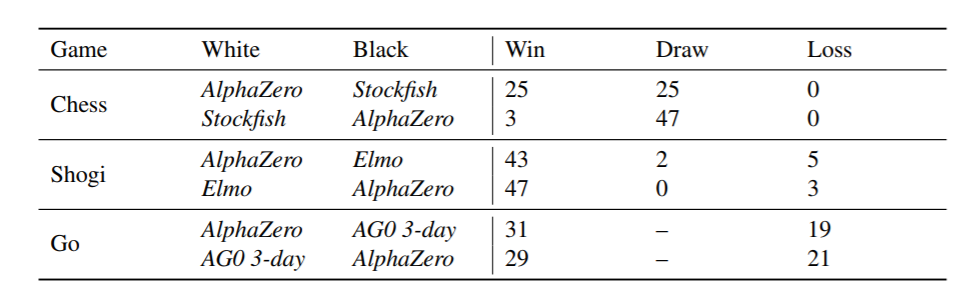
\includegraphics[width=16cm,height=7cm]{table.png}
	\caption{AlphaZero's Ergebnisse}
	\label{img:passante}
\end{figure}
\\
AlphaZeros Leistung im Schachbereich war überzeugen. So gewann er aus 100 Spielen 32 Partien und spielte 68 mal unentschieden. Dabei hatte AlphaZero 25 mal weiß. Der Gegner war Stockfish 8. Stockfish ist auch eine Schachengine, welche von Tord Romstad entwickelt wurde und lange die Weltrangliste der Engines anführte. Stockfish erkennt pro Zug 70 Millionen verschiedene Stellungen, AlphaZero legendlich 70 Tausend. Die Zugmatrizen bei AlphaZero sind einfacher und effizienter konzipiert, wodurch eine besseres lernen möglich ist. Es spielt nach jeden Zug eine Partie aus der Stellung heraus gegen sich selber und erkennt daran, ob der Zug \dq gut\dq\vspace{10px} oder \dq schlecht \dq ist. 
